\chapter{Algoritmos de Sumarização de Texto}
\label{cap:algoritmos}

Este capítulo, explica os algoritmos utilizados nessa monografia que, por meio de uma pesquisa, comparará cada um destes algoritmos consolidados com o proposto pelo autor do presente trabalho.

\section{Algoritmo de Luhn}
\label{chap:Algluhn}
O algoritmo de Luhn analisa as frases mais importantes de um documento, que são aquelas que mais aparecem no 
texto. Neste contexto, não são consideradas as \textit{stopwords}, que são palavras como artigos, preposições, 
conjunções, entre outras que aparecem com frequência em um texto, porém são insignificantes em relação ao 
significado semântico do documento \cite{da2022mineraccao}. Em suma, as \textit{stopwords} são utilizadas apenas 
para dar um sentido gramatical correto na formação das frases. Como o algoritmo faz a sumarização baseada na 
frequência que as palavras ocorrem, elas são desconsideradas para não confundir o sumarizador.

\begin{figure}
    \centering
    \caption{Modelo de Funcionamento do Algoritmo de Luhn}
    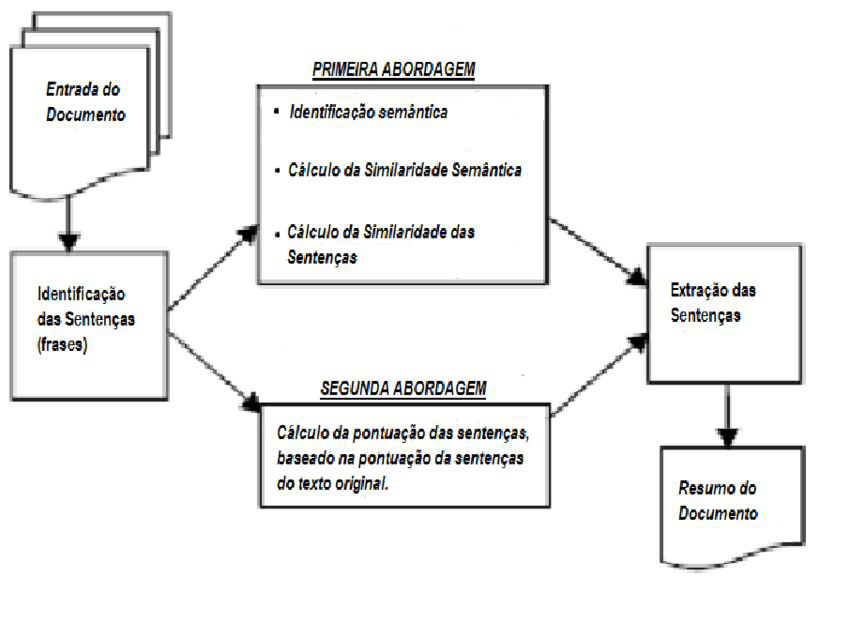
\includegraphics[width=.8\textwidth]{figuras/luhn-funcionamento.png}
    \Fonte{Extraído de \cite{russell2011mineraccao}.} 
    \label{fig:luhn-figure}
\end{figure}

O algoritmo não procura compreender os dados em um nível semântico, e simplesmente computa resumos com 
agrupamento de palavras que ocorrem com frequência no texto. A Figura \ref{fig:luhn-figure} apresenta os 
passos desde quando o algoritmo de Luhn recebe um texto como parâmetro até a geração final do resumo. A 
primeira tarefa é identificar as frases, calculando a similaridade entre todas as frases do texto. Na 
segunda abordagem, outra tarefa é fazer o cálculo da pontuação, levando em conta que o resumo nunca pode ter 
mais pontos e vírgulas que o texto original. Terminadas a primeira e segunda abordagens mostradas na Figura 
\ref{fig:luhn-figure}, o algoritmo finalmente extrai as sentenças escolhidas, as agrupa e mostra como resultado o resumo. O resumo gerado pelo algoritmo de Luhn está no anexo \ref{chap:luhn_resumo}

O algoritmo de Regressão Bayesiana é uma releitura do Algoritmo de Luhn, funcionando conforme descrito anteriormente. O resumo gerado pelo algoritmo de Regressão Bayesiana está no anexo \ref{chap:bayesiana_resumo}.


\section{Algoritmo Gistsumm}
\label{chap:Alggistsumm}
O \textit{GistSumm} (\textit{GistSumarizer}) é um sumarizador extrativo que usa técnicas estatísticas para determinar a ideia central dos textos por ele sumarizados. Baseia-se na simulação da sumarização humana, primeiro identificando a ideia principal do texto e, então, acrescenta informações adicionais ou complementares \cite{brewka1996artificial}. Essas informações adicionais podem ser a segunda ou terceira frase mais importante do texto, seguindo em ordem crescente de acordo com a quantidade de frases que se deseja extrair do texto.

Dessa forma, o sumarizador primeiro procura a sentença que melhor expressa a ideia principal do texto e baseado nela são escolhidas as demais sentenças, que vão compor o extrato textual. Mesmo quando a sentença escolhida não for a sentença principal e há uma aproximação significativa da mesma, o extrato já pode ser gerado \cite{torres2014automatic}. 

O \textit{GistSumm} compreende três processos principais, e mais alguns secundários, os quais são descritos a seguir: segmentação textual, ranqueamento de sentenças e seleção de sentenças.

A segmentação textual delimita as sentenças do texto-fonte e procura pelos sinais de pontuação. O ranqueamento é uma ordenação a partir de pesos obtidos na aplicação de métodos estatísticos, sendo feita a análise léxica, extração das \textit{stopwords} e aplicação do método de ranqueamento. Por fim, a seleção de sentença escolhe as sentenças mais relevantes, por meio de seus métodos extrativos, para, deste modo, gerar o sumário do documento analisado \cite{muller2015comparativo}. Neste momento, o texto é transformado de acordo com a taxa de compressão definida. A taxa de compressão é a porcentagem do texto original que o algoritmo pode extrair para o resumo.
O resumo gerado pelo algoritmo \textit{Gistsumm} está no anexo \ref{chap:gistsumm_resumo}.


\section{Algoritmo de Programação Linear Inteira (PLI)}
\label{sec:algoritmo-oliveira}

O Algoritmo de programação Linear Inteira tem como objetivo a sumarização automática de textos baseada em conceitos, utilizando programação linear inteira e regressão. Essa abordagem busca extrair as informações mais importantes de um texto e gerar um resumo coerente e relevante. O PLI segue as etapas:

\subsection{Pré-processamento}
Nesta etapa, o texto é pré-processado para eliminar ruídos e facilitar a extração de informações. O pré-processamento inclui a remoção de pontuação, números, caracteres especiais e \textit{stopwords}, além da normalização do texto, como a conversão de todas as letras para minúsculas e a redução das palavras ao seu radical (\textit{stemming}).

\subsection{Extração de Conceitos}
Com base no texto pré-processado, os conceitos são extraídos. Um conceito é uma palavra ou expressão que representa uma ideia importante no texto. A frequência de cada conceito no texto é calculada, e os conceitos são ordenados de acordo com sua importância, considerando suas frequências e pesos semânticos.

\subsection{Seleção de Sentenças}
Nesta etapa, as sentenças que contêm os conceitos mais importantes são selecionadas para compor o resumo. O algoritmo utiliza programação linear inteira para determinar a melhor combinação de sentenças que maximiza a cobertura dos conceitos importantes, mantendo a coerência e a concisão do resumo. A programação linear inteira é uma técnica matemática que permite a resolução de problemas de otimização com variáveis inteiras.

\subsection{Regressão}
A regressão é aplicada para ajustar os pesos dos conceitos e das sentenças, de forma a melhorar a qualidade do resumo gerado. O algoritmo utiliza um conjunto de treinamento com textos e resumos previamente avaliados por humanos para aprender a importância relativa dos conceitos e sentenças no processo de sumarização. A regressão permite que o algoritmo ajuste seus parâmetros de acordo com os padrões observados nos dados de treinamento, melhorando a precisão e a relevância dos resumos gerados.

\subsection{Geração do Resumo}
Com base na seleção de sentenças e nos pesos ajustados dos conceitos, o resumo final é gerado. As sentenças selecionadas são reorganizadas de acordo com a ordem em que aparecem no texto original, garantindo a coerência e a fluidez do resumo.

O PLI apresenta uma abordagem interessante para a sumarização automática de textos, combinando técnicas de programação linear inteira e regressão para extrair e ponderar conceitos importantes e selecionar as sentenças mais relevantes para compor o resumo. Essa abordagem busca gerar resumos mais precisos, coerentes e informativos, levando em consideração a importância dos conceitos e a estrutura do texto original.
O resumo gerado está no anexo \ref{chap:pli_resumo}.


\section{\textit{ChatGPT}}
\label{chap:chatgpt}

O \textit{ChatGPT} é um algoritmo baseado em inteligência artificial, criado pela \textit{OpenAI} \cite{lund2023chatting}. Seu nome vem é uma sigla de \textit{Generative Pre-Trained Transformer}, que significa, em tradução livre, Transformador pré-treinado generativo \cite{transformer2022rapamycin}. Esse algoritmo tem seu desenvolvimento traçado a partir de redes neurais e \textit{Machine Learning}, e tem foco semelhante a \textit{chatbots}, com conversação online. A ideia a partir do que ele foi criado, é para aprimorar a experiência e recursos oferecidos por alguns assistentes virtuais, como Alexa, Google Assistente, dentre outros. Grande parte de ter se tornado famoso e ter tanto sucesso se dá pela forma simples de conversação e obtenção de respostas \cite{aydin2023ChatGPT}.

A sua arquitetura se baseia em uma rede neural chamada \textit{Transformer}, que é projetada especialmente para lidar com textos. Seu modelo de várias camadas permite que a plataforma consiga identificar palavras-chave, nos mais diferentes contextos inseridos \cite{natarajan2020wide}. Esse algoritmo se alimenta de informações que colhe da Internet. Nesse caso, tudo que existe hoje disponível na rede pode ser usado como base para essa ferramenta \cite{rao2023assessing}. Seguindo alguns padrões e no cruzamento de informações, o \textit{ChatGPT} transforma as \textit{querys}, perguntas feitas pelo usuário, em respostas. Seu diferencial se dá na criatividade que está presente nessas respostas, já que, diferente dos métodos tradicionais de busca, ele traz a resposta contextualizada e em um texto elaborado que busca o maior entendimento do leitor, além da possibilidade de elaborar musicas, poesias, códigos de programação, receitas, dentre outras \cite{rudolph2023chatgpt}.
O resumo gerado pelo \textit{ChatGPT} está no anexo \ref{chap:chatgpt_resumo}.


\section{Algoritmo de Marques}
\label{chap:marques}
O algoritmo proposto pelo autor tem embasamento no algoritmo \textit{GistSumm} (\textit{GistSumarizer}), que é embasado no algoritmo de Luhn, e seu método de extração de palavras-chave baseado na sentença principal do texto é muito eficiente quando trata-se de gerar resumos com as ideias principais de um texto \cite{castro2022extraccao}. De acordo com \citeonline{rino2003sumarizaccao}, o \textit{GistSumm} atualmente encontra-se como o estado da arte de sumarização automática de documentos, com uma função para sumarização multi-documentos.

Segundo o trabalho de \citeonline{de2011blmsumm}, a eficiência de um algoritmo de sumarização está ligada ao desempenho de seu método de extração de palavras-chave. Para verificar essa hipótese, serão utilizadas tabelas com os resultados, essas tabelas mostram todos os dados tanto em forma numérica e percentual, onde podemos perceber a eficiência e demais características dos algoritmos, tais como taxa de erros e acertos. Avaliações de forma semelhante a essas foram feitas nos trabalhos de Luhn e \citeonline{rino2003sumarizaccao}, sendo que somente o trabalho de \citeonline{rino2003sumarizaccao} aplica-se ao português do Brasil.

O algoritmo de Marques é um sumarizador extrativo que usa técnicas estatísticas para determinar a ideia central dos textos por ele sumarizados, que implementa bibliotecas da linguagem \textit{Python} 3.10. Baseia-se na simulação da sumarização humana, primeiro identificando a ideia principal do texto e, então, acrescenta informações adicionais ou complementares. Essas informações adicionais podem ser a segunda ou terceira frase mais importante do texto, seguindo em ordem crescente de acordo com a quantidade de frases que se deseja extrair do texto.

Dessa forma, o sumarizador primeiro procura a sentença que melhor expressa a ideia principal do texto, e baseado nela são escolhidas as demais sentenças que vão compor o extrato textual. O \textit{GistSumm} trabalha da mesma forma: primeiro o GistSumm realiza a identificação da sentença principal com o uso de métodos estatísticos simples, e, por segundo, conhecendo-se as sentenças principais é possível produzir extratos coerentes. Mesmo quando a sentença escolhida não for a sentença principal e há uma aproximação significativa da mesma, o extrato já pode ser gerado.
O código do algoritmo de Marques está no apêndice \ref{chap:marques_algoritmo}.
O resumo gerado pelo algoritmo de Marques está no apêndice \ref{chap:marques_resumo}.